
\section{The Impact of Input Complexity on Tempotron Performance}

\subsection{Experimental Framework}

The primary objective of this investigation is to evaluate the performance trajectory of the Tempotron model in response to varying degrees of input complexity. The complexity measure, \( \alpha \), represents the ratio of distinct spike patterns \( P \) to the total number of input neurons \( N \):
\[ \alpha = \frac{P}{N} \]


\subsection{Input Data Synthesis}

Spike sequences were generated to ensure each neuron emits a solitary spike at random intervals, creating a myriad of unique patterns as governed by the \( \alpha \) ratio.

\subsection{Model Architecture}

The Tempotron model's design and operational mechanics are primarily defined in \ref{st:GD-simple-medel}


\subsection{Procedure}

For each selected \( \alpha \) value, multiple experimental trials were executed, each undergoing a preset number of learning iterations, processing data in specified batch sizes.



\subsection{Parameter Descriptions}

\begin{enumerate}
    \item \textbf{Duration \( T \): 500 ms} \\
    Represents the length of time for which the model will simulate the neural dynamics for each given input pattern.
    
    \item \textbf{Time step \( dt \): 1 ms} \\
    The sampling time at which we "measure" the experiment.
    
    \item \textbf{Resting potential \( V_0 \): 2.12} 
    
    \item \textbf{Firing threshold \( V_{th} \): 1} \\
    The potential level at which a neuron emits a spike. When the neuron's membrane potential exceeds \( V_{th} \), it "fires" or produces an output spike.
    
    \item \textbf{Time constant \( \tau \): 10 ms} \\
    Determines the rate at which a neuron's membrane potential decays back towards its resting potential after perturbation.
    
    \item \textbf{Output layer size: 1 neuron} \\
    Indicates the number of neurons in the model's final layer, which produces the final decision or classification.
    
    \item \textbf{Maximum iterations: 750} 

    \item \textbf{Batch size: 64} \\
    Dictates how many input patterns are processed simultaneously before updating the model's internal parameters. 

\end{enumerate}

\subsection{Results}

\begin{figure}[H]
    \centering
    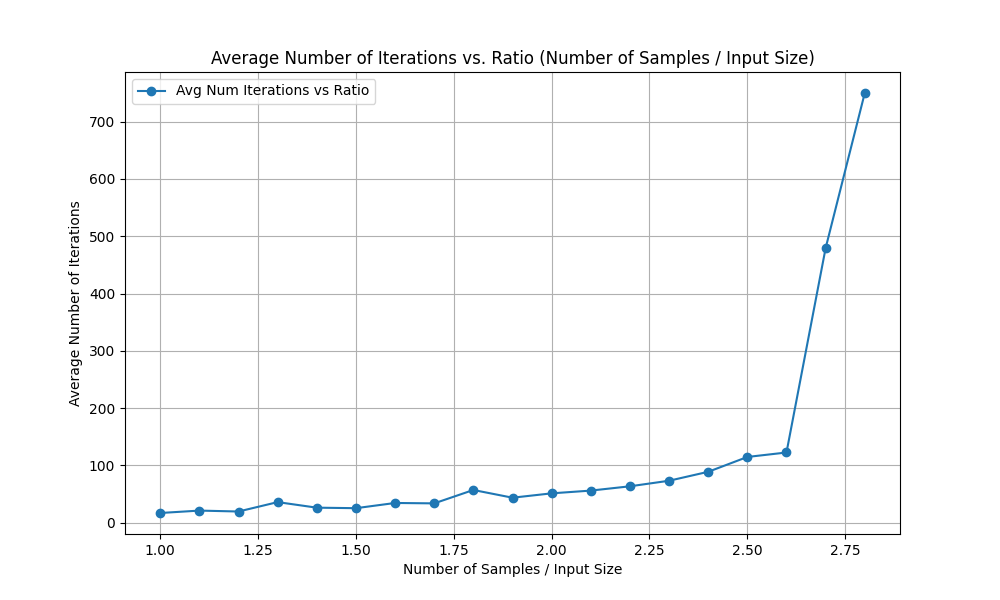
\includegraphics[width=0.8\linewidth]{results/graphs/alpha-validation.png}
    \caption{Number of training iterations until 100\% accuracy on the training data as a function of the ratio between the number of patterns and the input size}
    \label{fig:alpha-validation}
\end{figure}


\section{Observation}

The data collected from the experiment showcases the relationship between the ratio (\( \alpha \)) of different input patterns to neurons in the input layer and the average number of iterations required for the Tempotron to converge.

\textbf{Extreme Complexity Region (\( \alpha \geq\) 2.9)}: \\
Notably, at \( \alpha = 2.8 \), the average epochs reach the maximum value of 750, which was our defined limit. This may hint at a failure to converge, indicating that the Tempotron finds it virtually impossible to discern patterns at such high complexities using the given parameters.

Several factors might contribute to these observations:

\begin{itemize}
    \item The inherent design of the Tempotron, which relies on the temporal dynamics of spikes, may find it challenging to discriminate between overlapping or similar spike patterns as \( \alpha \) grows.
    
    \item The fixed parameters, such as the firing threshold \( V_{th} \) or the time constant \( \tau \), may not be optimal for handling higher complexity ratios. Adaptive mechanisms or parameter tuning might be necessary for such scenarios.
    
\end{itemize}

In conclusion, the Tempotron exhibits strong performance in classifying time-dependent, its capability goes beyond the recognized limit of \( \alpha = 2 \) for a single-layer perceptron \cite{gutig2006tempotron}. This fact is a strong foundation on which we rely our hipthesis that the Tempotron holds significant structural and ? benefits over the perceptron

In conclusion, the Tempotron demonstrates strong performance in classifying time-dependent patterns. Remarkably, its capacity surpasses the recognized threshold of \( \alpha = 2 \) associated with a single-layer perceptron \cite{gutig2006tempotron}. This observation forms a basis for our hypothesis that the Tempotron offers substantial structural and functional advantages over the perceptron.
